\documentclass[varwidth=true, border=2pt]{standalone}

\usepackage{pgfplots}
\usepackage{tikz}

\usetikzlibrary{calc,patterns,angles,quotes,spy}

\begin{document}
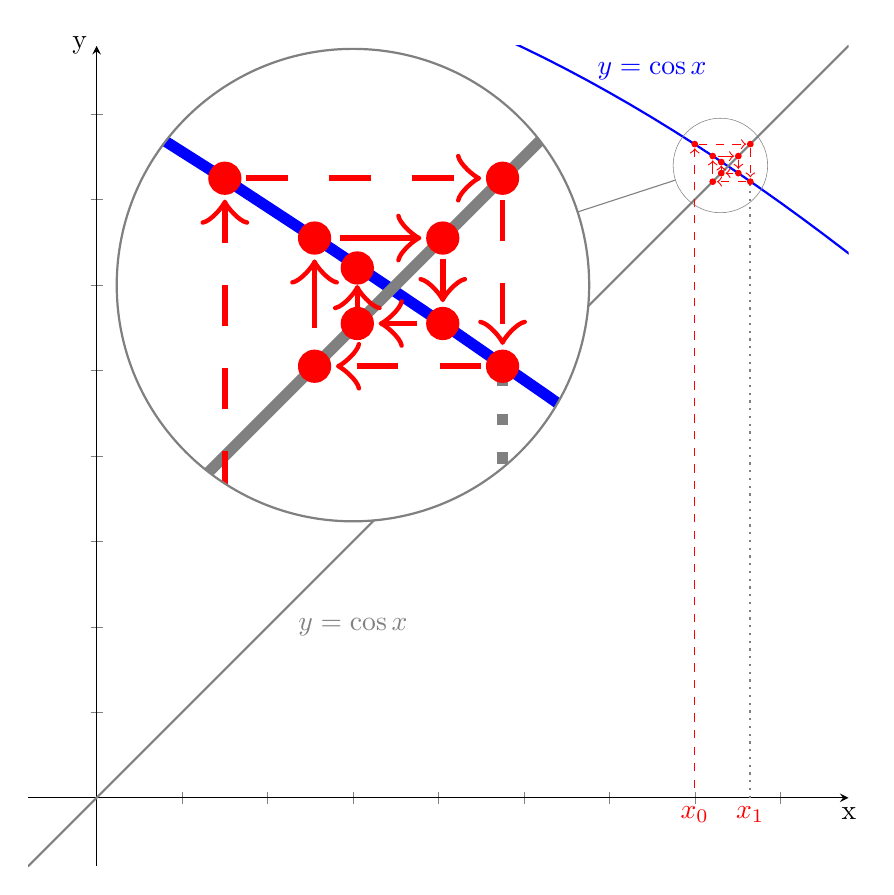
\begin{tikzpicture}[spy using outlines=
	{circle, magnification=5, connect spies}]
    \begin{axis}[
        legend pos=south east,
        axis x line=middle,
        axis y line=middle,
	every axis x label/.style={at={(current axis.right of origin)},anchor=north},
	every axis y label/.style={at={(current axis.above origin)},anchor=east},
	xticklabels=\empty,
	yticklabels=\empty
        grid = none,
        width=12cm,
        height=12cm,
        grid style={dashed, gray!1},
        xmin=0,     % start the diagram at this x-coordinate
        xmax= 0.8,    % end   the diagram at this x-coordinate
        ymin=0,     % start the diagram at this y-coordinate
        ymax= 0.8,   % end   the diagram at this y-coordinate
        xlabel=x,
        ylabel=y,
        enlargelimits=true,
        tension=0.08]

        \addplot[domain=-1.57:4.71,blue, thick,samples=250] {cos(deg(x))};
        \addplot[domain=-1:2, gray, thick,samples=250] {x};



	
	\addplot[red, only marks, mark=*, mark size=1pt] coordinates {(0.7,0.765)(0.765,0.765)(0.765, 0.721)(0.721,0.721)(0.721,0.751)(0.751,0.751)(0.751,0.731)(0.731,0.731)(0.731,0.744)};
	\node(cX)[blue] at (axis cs: 0.65,0.85){{$y = \cos x  $}};
	\node(yX)[gray] at (axis cs: 0.3,0.2){{$y = \cos x  $}};


	\node[red] (y0) at (axis cs: 0.7,0){};
	\node[red] (x0) at (axis cs: 0.7,0.765){};
	\node[red] (y1) at (axis cs: 0.765,0.765){};
	\node[red] (x1) at (axis cs: 0.765,0.721){};
	\node[red] (y2) at (axis cs: 0.721,0.721){};
	\node[red] (x2) at (axis cs: 0.721,0.751){};
	\node[red] (y3) at (axis cs: 0.751,0.751){};
	\node[red] (x3) at (axis cs: 0.751,0.735){};
	
	\node[red] (x_0) at (axis cs: 0.7, -0.02){$x_0$};
	\node[red] (x_1) at (axis cs: 0.765, -0.02){$x_1$};
	\addplot[dotted,gray,thick,mark=none] coordinates{(0.765,0)(0.765,0.721)} node[below, pos=0] {}; %x0
		
	\draw[red, dashed, ->](y0)--(axis cs: 0.7, 0.76);
	\draw[red, dashed, ->](axis cs: 0.705,0.765)--(axis cs: 0.76, 0.765);
	\draw[red, dashed, ->](axis cs: 0.765, 0.76)--(axis cs: 0.765, 0.726);
	\draw[red, dashed, ->](axis cs: 0.76, 0.721)--(axis cs: 0.726, 0.721);
	\draw[red, ->](axis cs: 0.721, 0.73)--(axis cs: 0.721, 0.746);
	\draw[red, ->](axis cs: 0.727, 0.751)--(axis cs: 0.746, 0.751);
	\draw[red, ->](axis cs: 0.751,0.746)--(axis cs: 0.751, 0.736);
	\draw[red, ->](axis cs:0.745,0.731)--(axis cs: 0.736, 0.731);
	\draw[red, ->](axis cs:0.731,0.731)--(axis cs: 0.731, 0.74);
		
	\coordinate (spypoint) at (axis cs:0.73,0.74);
	\coordinate (magnifyglass) at (axis cs:0.3,0.6);
	
	\spy [gray, size=6cm] on (spypoint)
   in node[fill=white] at (magnifyglass);
    \end{axis}
\end{tikzpicture}





\end{document}